%book template given by EG Goodaire: http://www.math.mun.ca/~edgar/thesis.html --Thanks!
\documentclass[11pt]{book} 
\usepackage{amsmath} %Never write a paper without using amsmath for its many new commands 
\usepackage{amssymb} %Some extra symbols 
%\usepackage{makeidx} %If you want to generate an index, automatically 
\usepackage{graphicx,caption} %If you want to include postscript graphics 
\usepackage{mystyle} %Create your own file, mystyle.sty where you put all your own \newcommand statements, for example. 

%\includeonly{chaptr2} %If you just want to process chaptr2.tex 


\begin{document} 

%inspired by http://en.wikibooks.org/wiki/LaTeX/Title_Creation#A_practical_example
\begin{titlepage}
\begin{center}

% Upper part of the page. The '~' is needed because \\
% only works if a paragraph has started.
\noindent\begin{minipage}{.4\textwidth}
\centering

\includegraphics[width=\linewidth]{./img/uva-logo.png}~\\[.5cm]
\textsc{\normalsize University of Virginia}\\[1.5cm]
\end{minipage}
\hfill
\noindent\begin{minipage}{.4\textwidth}
\centering

\includegraphics[width=\linewidth]{./img/duke-logo.png}~\\[.5cm]
\textsc{\normalsize Duke University}\\[1.5cm]
\end{minipage}
\\[80pt]
\textsc{\Large HiFrost Reference Manual}\\[0.5cm]

% Title
\HRule \\[0.4cm]
{ \huge \bfseries The HI$\gamma$S Frozen Spin Target \\[0.4cm] }

\HRule \\[1.5cm]

% Author and supervisor
\begin{minipage}{0.4\textwidth}
\begin{flushleft} \large
\emph{Author:}\\
Ryan \textsc{Duve}
\end{flushleft}
\end{minipage}
\begin{minipage}{0.4\textwidth}
\begin{flushright} \large
\emph{Supervisor:} \\
Blaine \textsc{Norum}
\end{flushright}
\end{minipage}

\vfill

% Bottom of the page
{\large \today}

\end{center}
\end{titlepage}
\pagestyle{empty} 
\chapter*{Preface}
\thispagestyle{empty} 


HiFrost is nuclear polarized target apparatus consisting of a dilution refrigerator, internal magnetic coil, microwave guide and NMR coil.  External components of HiFrost include a polarizing magnet, microwave generating EIO, pump and vacuum system to run the dilution refrigerator, and the Q-Meter/Yale Card set up for running the NMR. 


To polarize a target, chemically doped or irradiated beads are placed in the inner-most chamber, the fridge is assembled around the beads and the whole fridge is swung to align with the HIGS gamma beam.  The beads are cooled with liquid helium and polarized with a large external magnet, with an EIO providing microwaves necessary for dynamic nuclear polarization.


To achieve frozen spin mode, the internal magnet is ramped on as the external magnet is ramped off, so eventually the external magnet can be powered down and removed while keeping the polarized beads in a steady magnetic field. 
\frontmatter 
\tableofcontents 

\mainmatter 
\chapter{History} 
\label{history} % So I can \ref{altrings} later. 

\section{Polarized Targets}

\section{Inception}  
 
\section{CERN} 
 
\section{Geesthacht} 

\section{Virginia}

\section{Duke}
\chapter{Theory of Operation} 
\label{theory}  
\section{Nuclear Polarization}
In the presence of a magnetic field, spin-\half{} nuclei tend to align themselves along the axis of the field.  The polarization of the ensemble of particles is defined by 

$$P=\frac{\uparrow-\downarrow}{\uparrow+\downarrow},$$

where ($\downarrow$, $\uparrow$) is the population of nuclei with $m_z$=(-\half,\half).

\subsection{Thermal Polarization Derivation}

 \subsection{DNP}
Dynamic Nuclear Polarization (DNP) is a process of using microwave radiation to pump electron-proton pairs to higher energy (polarized) states.  The relaxation time for the electron is much shorter than that of the proton, so the proton remains polarized while the electron is able to be paired with other protons for polarization.

\begin{figure}
 \centering
 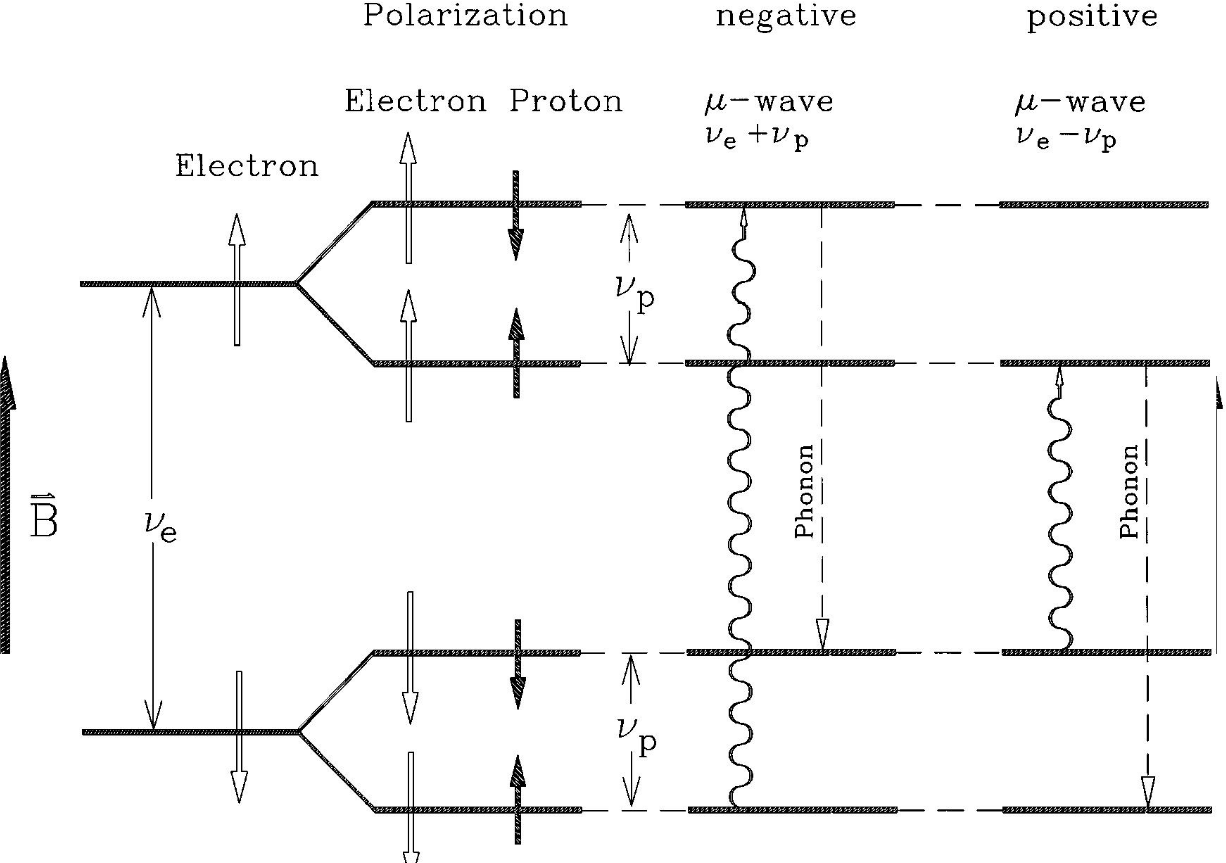
\includegraphics[scale=.25]{img/dnp.png}
 % dnp.png: 1226x863 pixel, 72dpi, 43.25x30.44 cm, bb=0 0 1226 863
 \caption{DNP diagram \cite{dnpdiagram}.  The white arrows are electron polarization and the black arrows are proton polarization.  Microwaves at a frequency difference $\nu_e\pm\nu_p$ flip the spins of both particles, and the electron's superior lattice coupling ensures it will flip back before the proton.}
 \label{fig:dnp-diagram}
\end{figure}


The microwave frequency can either be the sum of the proton and electron splitting frequency or the difference, depending on whether the nucleons are to be aligned with or against the magnetic field. 
\section{NMR}

Nuclear Magnetic Resonance (NMR) is the method we use to measure the polarization of the target material.  Essentially, a coil in the immediate vicinity of the target acts as the inductor in an LCR circuit, the inductance of which changes as a function of the magnetic susceptibility of the nuclei in the coil.  Since the magnetic susceptibility and polarization are related, the resonance frequency of the LCR circuit tell us information about the polarization of the target material\cite{qmeterbook}. 

\subsection{Liverpool Q-Meter}

\subsubsection{$\lambda$/2 Cable}

\subsubsection{Diode Detector}

\subsubsection{Phase Sensitive Detector and BRM}

\subsection{PDP}

\section{Frozen Spin} 
 
 The target is polarized in a 2.5 T field, called the polarizing field.  The target will lose all polarization in an environment free of magnetic field.  However, the detector cannot fit around the polarizing magnet, and the polarizing magnet would obstruct outcoming neutrons, anway).  To maintain polarization while the target is in the detector, an internal 0.5 T field is turned on inside the fridge and the polarizing magnetic is wound down and removed.  The 0.5 field, called the holding field, sufficiently maintains polarization of nucleons while the detector is moved aroud the target and data is taken.

\section{Refrigerator} 
Since the polarization goes like the inverse of temperature, colder environments make for better polarized targets.  In our case, we use a dilution refrigerator, one that mixes the two isotopes \het{} and \hef{} for cooling, to reach target temperatures below 0.1 K.

\subsection{\hef{}Cooling (Evaporator and Separator)}

\subsection{Dilution}

The dilution refrigerator principle relies on the splitting of a \het/\hef{} mixture into two distinct phases, a \het{} concentrated phase and a \het{} dilute phase.  The area labeled ``Two-phase region'' in Figure \ref{fig:dilutiondiagram} illustrates which mixtures, characterized by \het{} concentration, are inaccessible at which temperatures.  Since two distinct phases in thermal contact are always in or striving for thermodynamic equilibrium, changing the concentration of the dilute phase (by pumping \het{} out of it) will cause atoms from the concentrated phase to cross the phase boundary to restore balance.  Since the heat change of mixing (enthalpy difference between the dilute phase and concentrated phase) is positive, the \het{} crossing the phase boundary must absorb energy from the surrounding environment, which it does in the form of heat.\cite{hocktechniques}

\begin{figure}
 \centering
 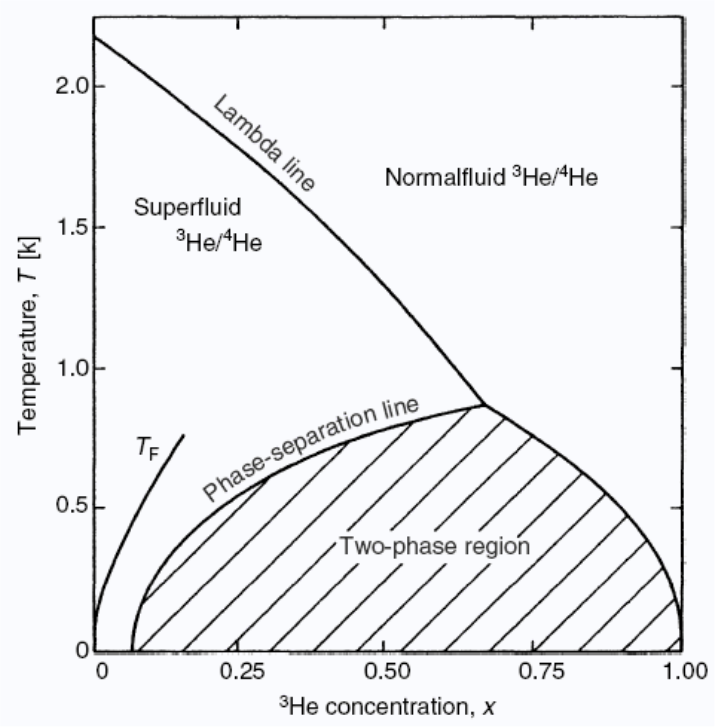
\includegraphics[scale=.45]{img/dilutiondiagram.png}
 % dilutiondiagram.png: 715x727 pixel, 72dpi, 25.22x25.64 cm, bb=0 0 715 727
 \caption{The famous diagram that shows the splitting of two distinct phases of $\het$-$\hef$ mixture. \cite{dilutiondiagram}}
 \label{fig:dilutiondiagram}
\end{figure}
 

\chapter{Fridge Tools}
\label{fridge-tools} 
\section{tools}
tools!
\subsection{small tools}
screw drivers
\subsection{big tools}
da fridge 
\chapter{Alternative Rings} 
\label{altrings} % So I can \ref{altrings} later. 
\section{Definitions} 
\label{defs} 
%\input{chap1/sec11} 
\section{The Cayley Numbers} 
\label{cayley} 
%\input{chap1/sec12} 
\section{Zorn's Vector Matrix Algebra} 
\label{zorn}  
%\include{chaptr3} 
%\include{chaptr4} 
%\include{chaptr5} 

\backmatter 
%\include{glossary} 
%\include{notat} 
%\bibliographystyle{amsalpha} %The style you want to use for references. 
%\bibliography{mr,refs} %The files containing all the articles and books you ever referenced. 
%\printindex %Make an index AUTOMATICALLY 

\end{document} ********End of master.tex 